\documentclass{beamer}
\usepackage[utf8]{inputenc}
\usepackage[normalem]{ulem}
\usepackage{tikz}
\usepackage{graphicx}
\usepackage{mathtools}
\DeclarePairedDelimiter{\ceil}{\lceil}{\rceil}
\usepackage{adjustbox}

\title{The \sout{Antibac}Buggy}
\author{Kent Odde, Stian Onarheim, Tarald Vestbøstad}
\institute{USN}
\date{Autumn 2020}

\begin{document}

\frame{\titlepage}
\addtobeamertemplate{headline}{}{%
    \begin{tikzpicture}[remember picture,overlay]
        \node at([shift={(.45\paperwidth,-.64)}]current page.north) {
\includegraphics[height=.5cm]{img/logo.png}};
    \end{tikzpicture}}

    \begin{frame}
        \frametitle{Showcase}
        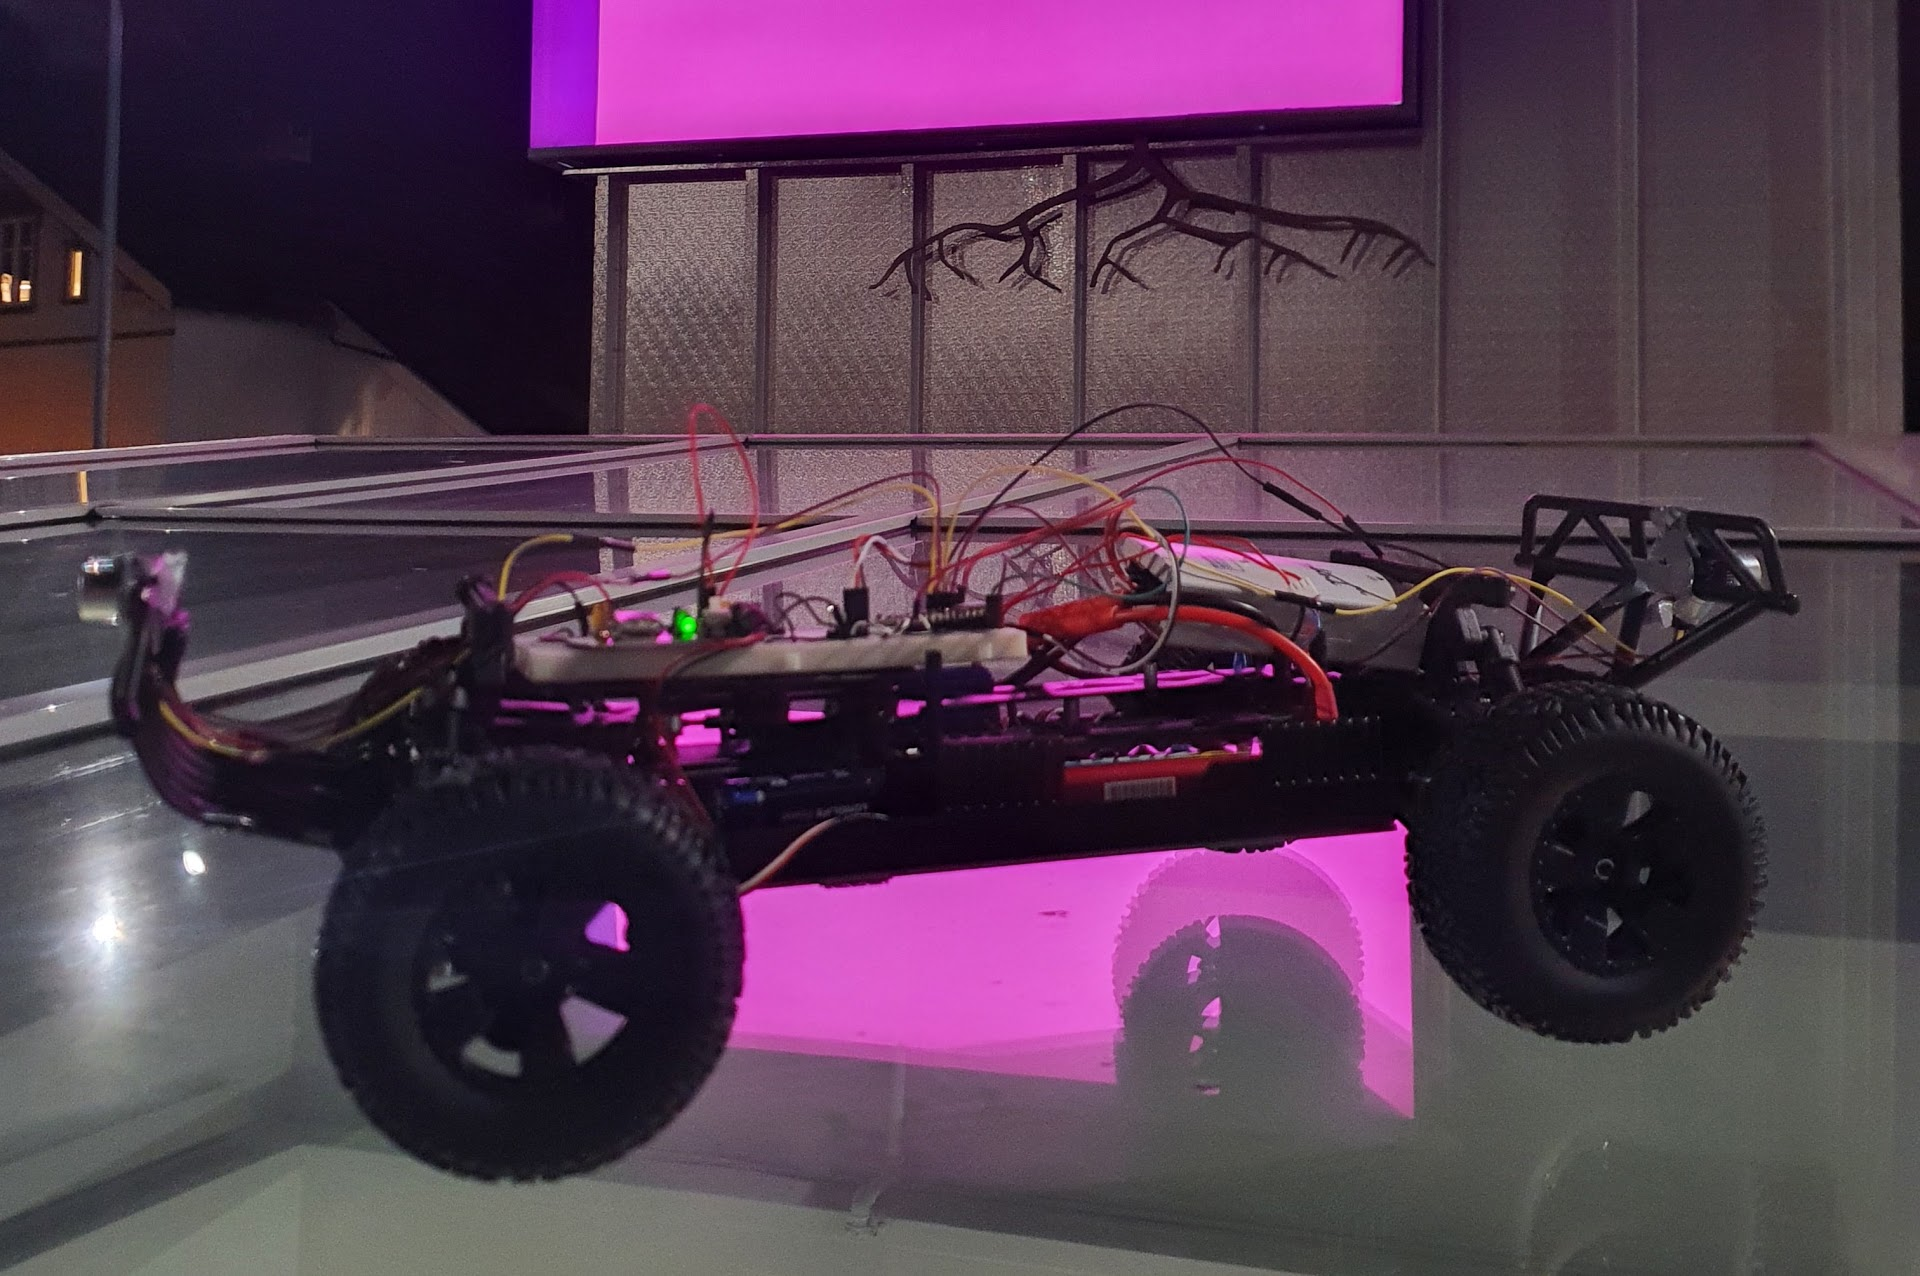
\includegraphics[width=\linewidth]{img/showcase.png}
    \end{frame}

    \begin{frame}
        \centering
        \frametitle{Initial Concept}
        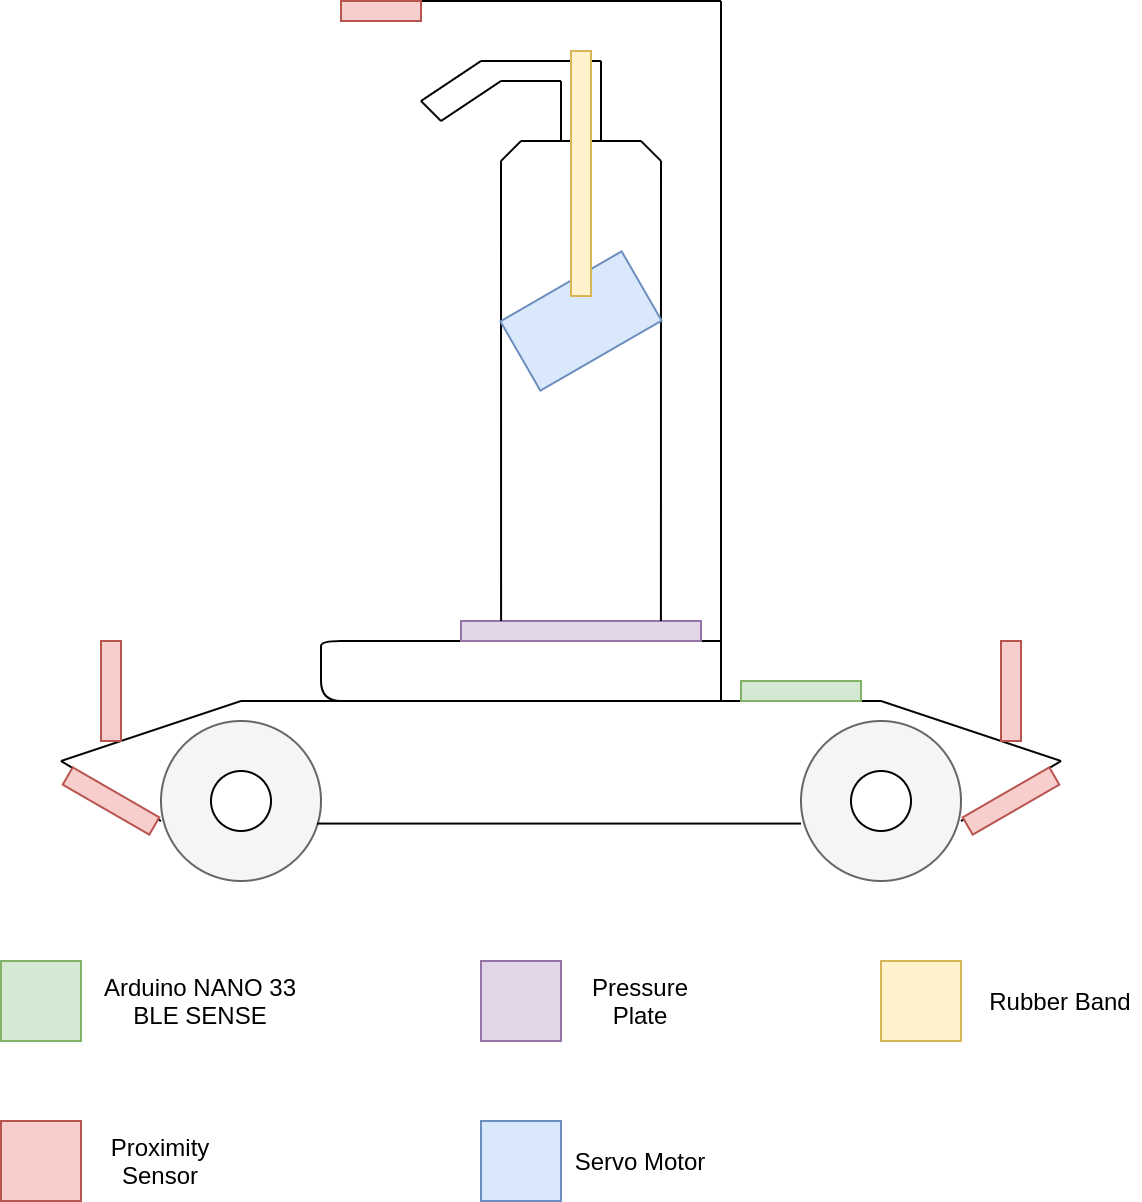
\includegraphics[scale=0.2, keepaspectratio]{img/prototype-drawing.png}
    \end{frame}

    \begin{frame}
        \frametitle{Timeline}
        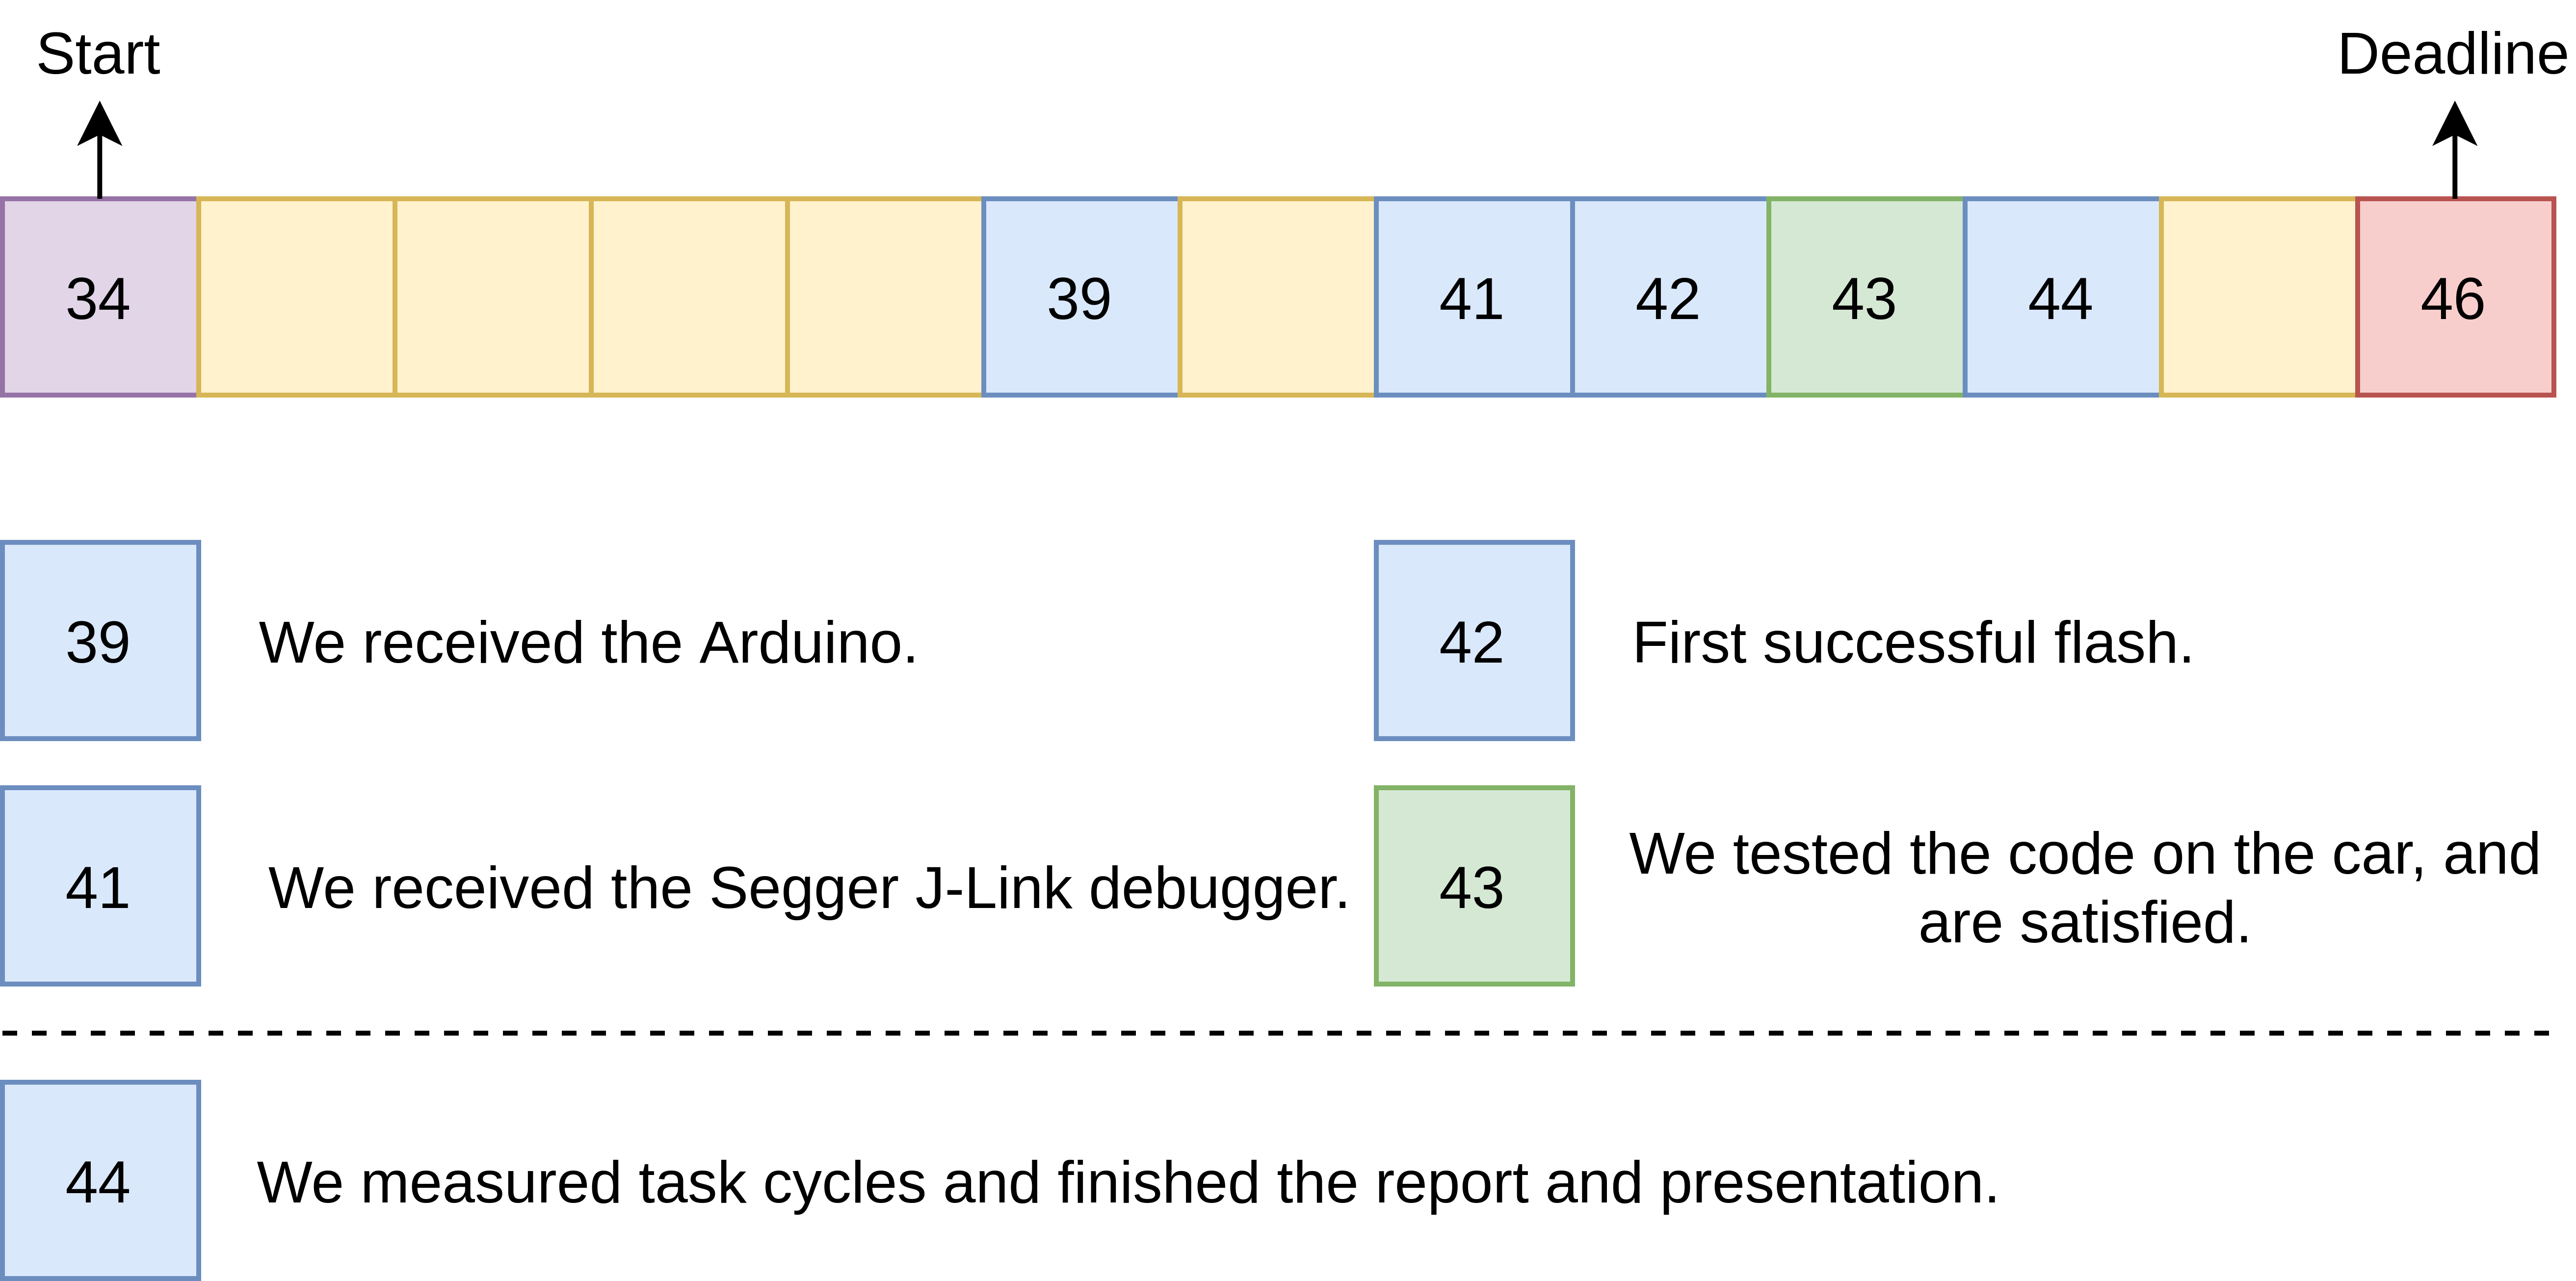
\includegraphics[width=\linewidth]{img/timeline.png}
    \end{frame}

    \begin{frame}
        \frametitle{Final Design}
        \centering
        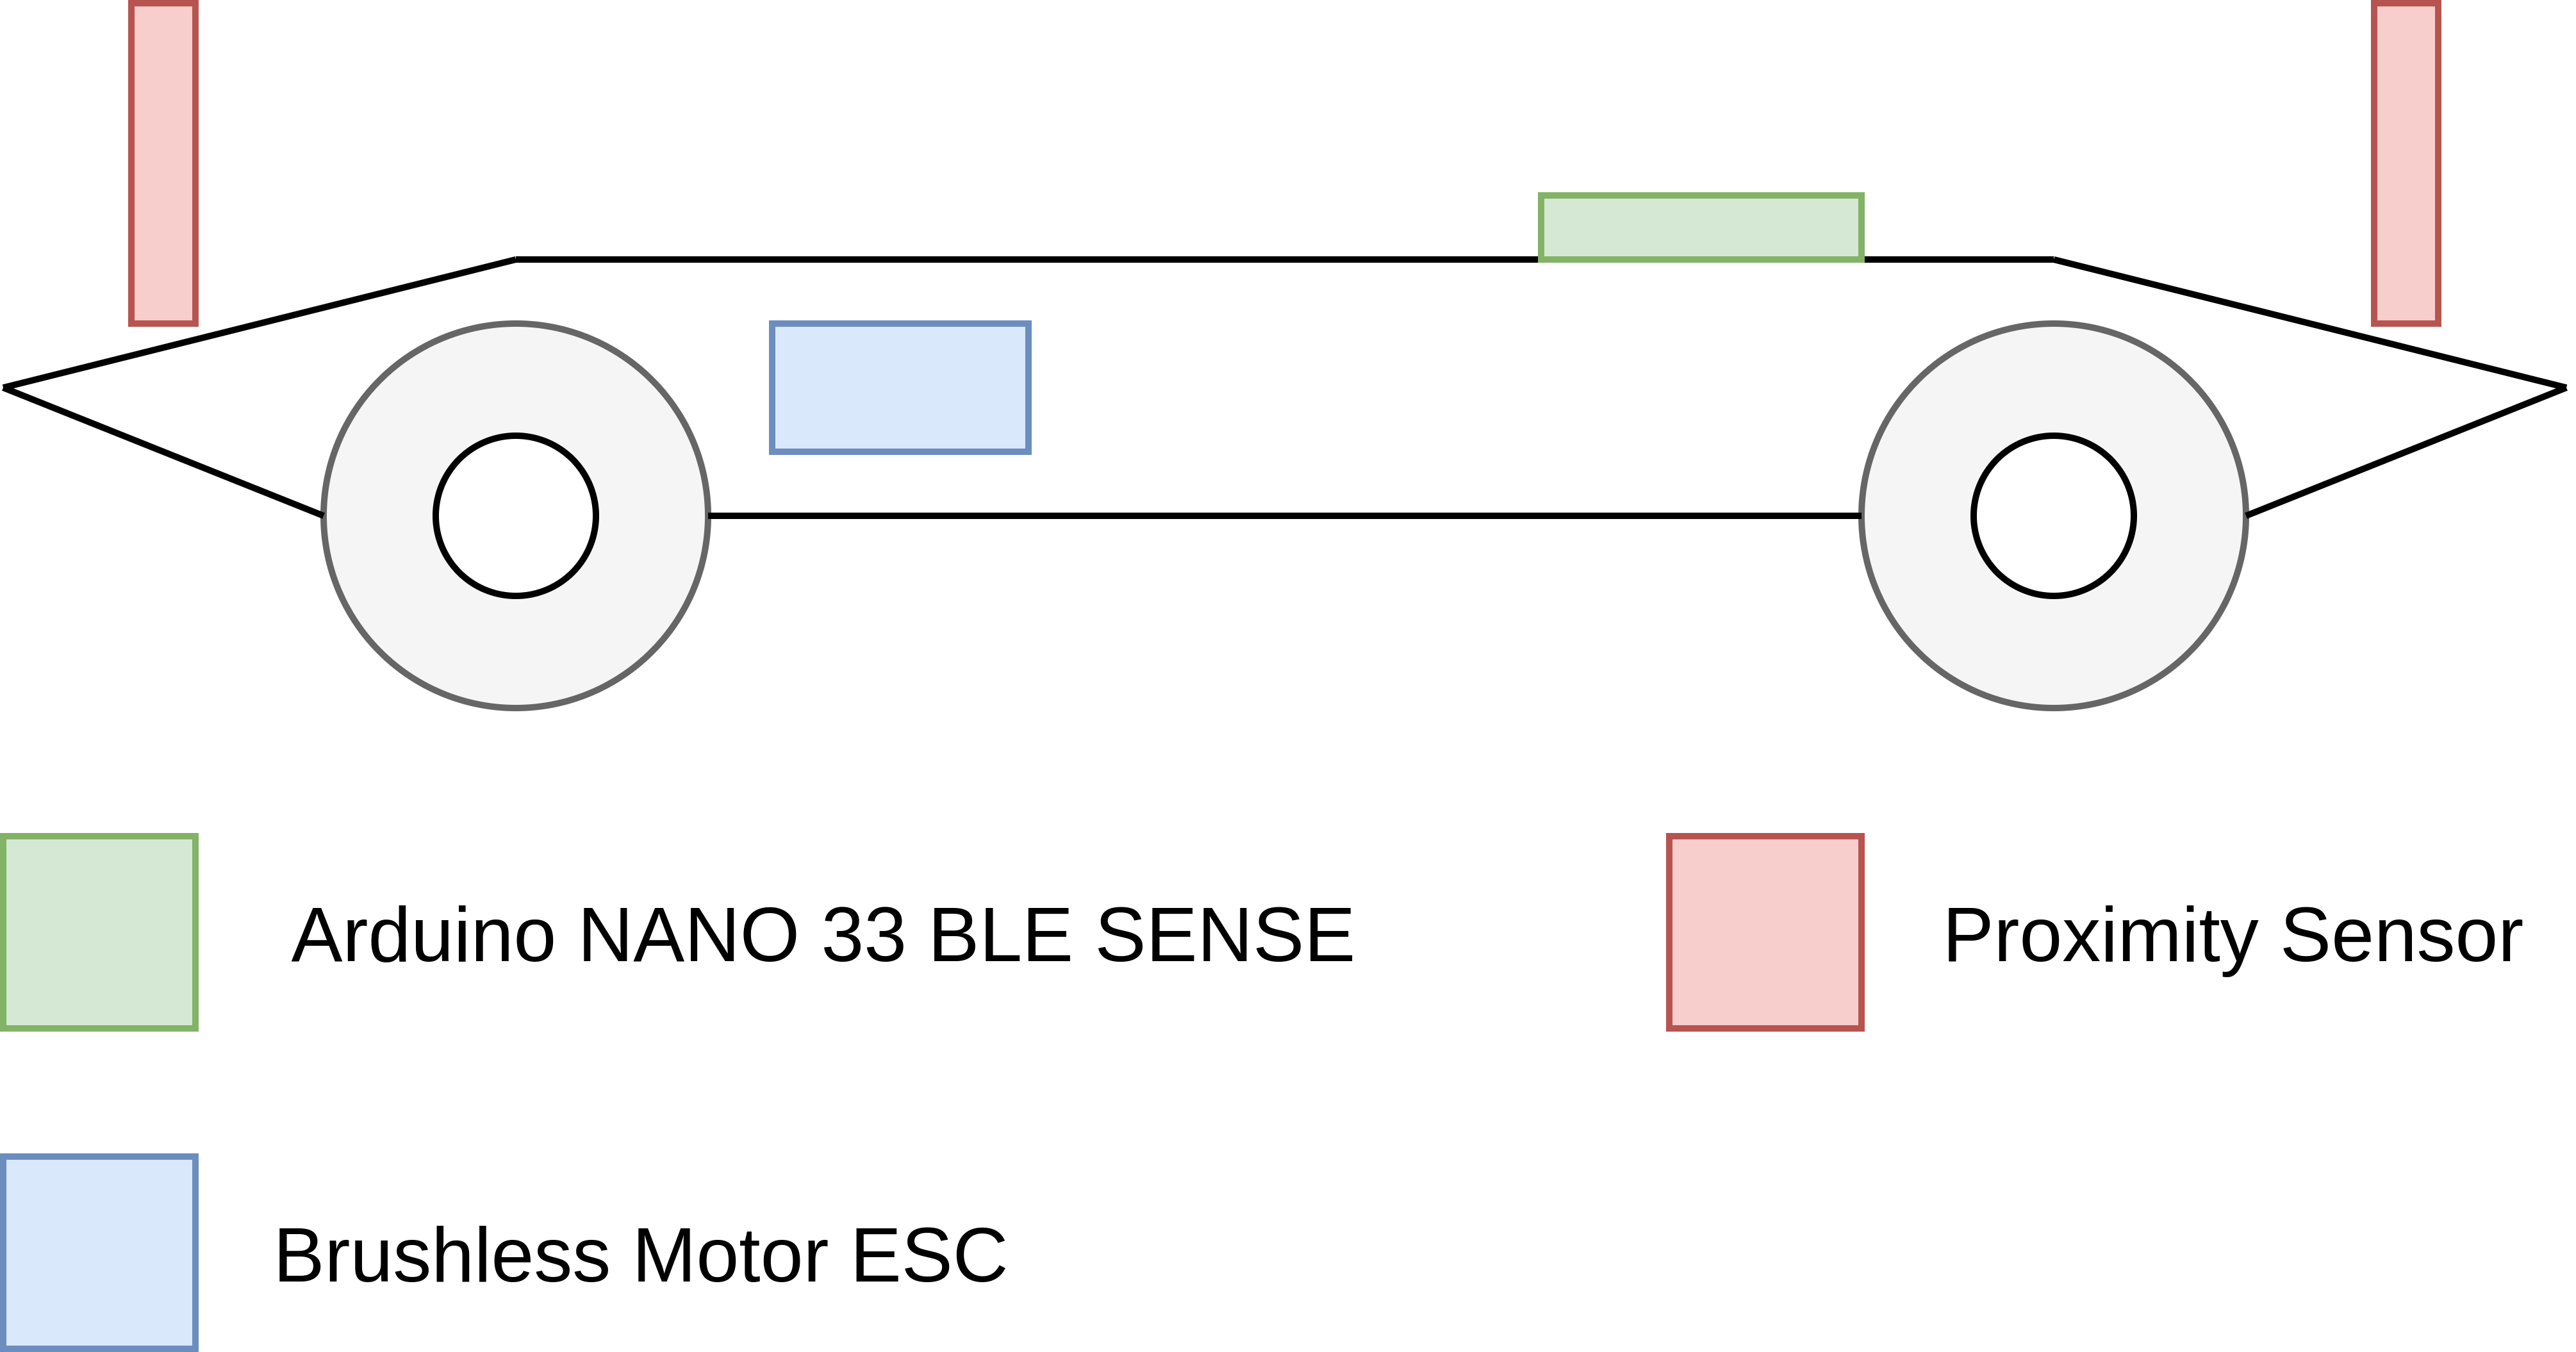
\includegraphics[scale=0.065]{img/final-design.png}
    \end{frame}

    \begin{frame}
        \frametitle{Servo}
        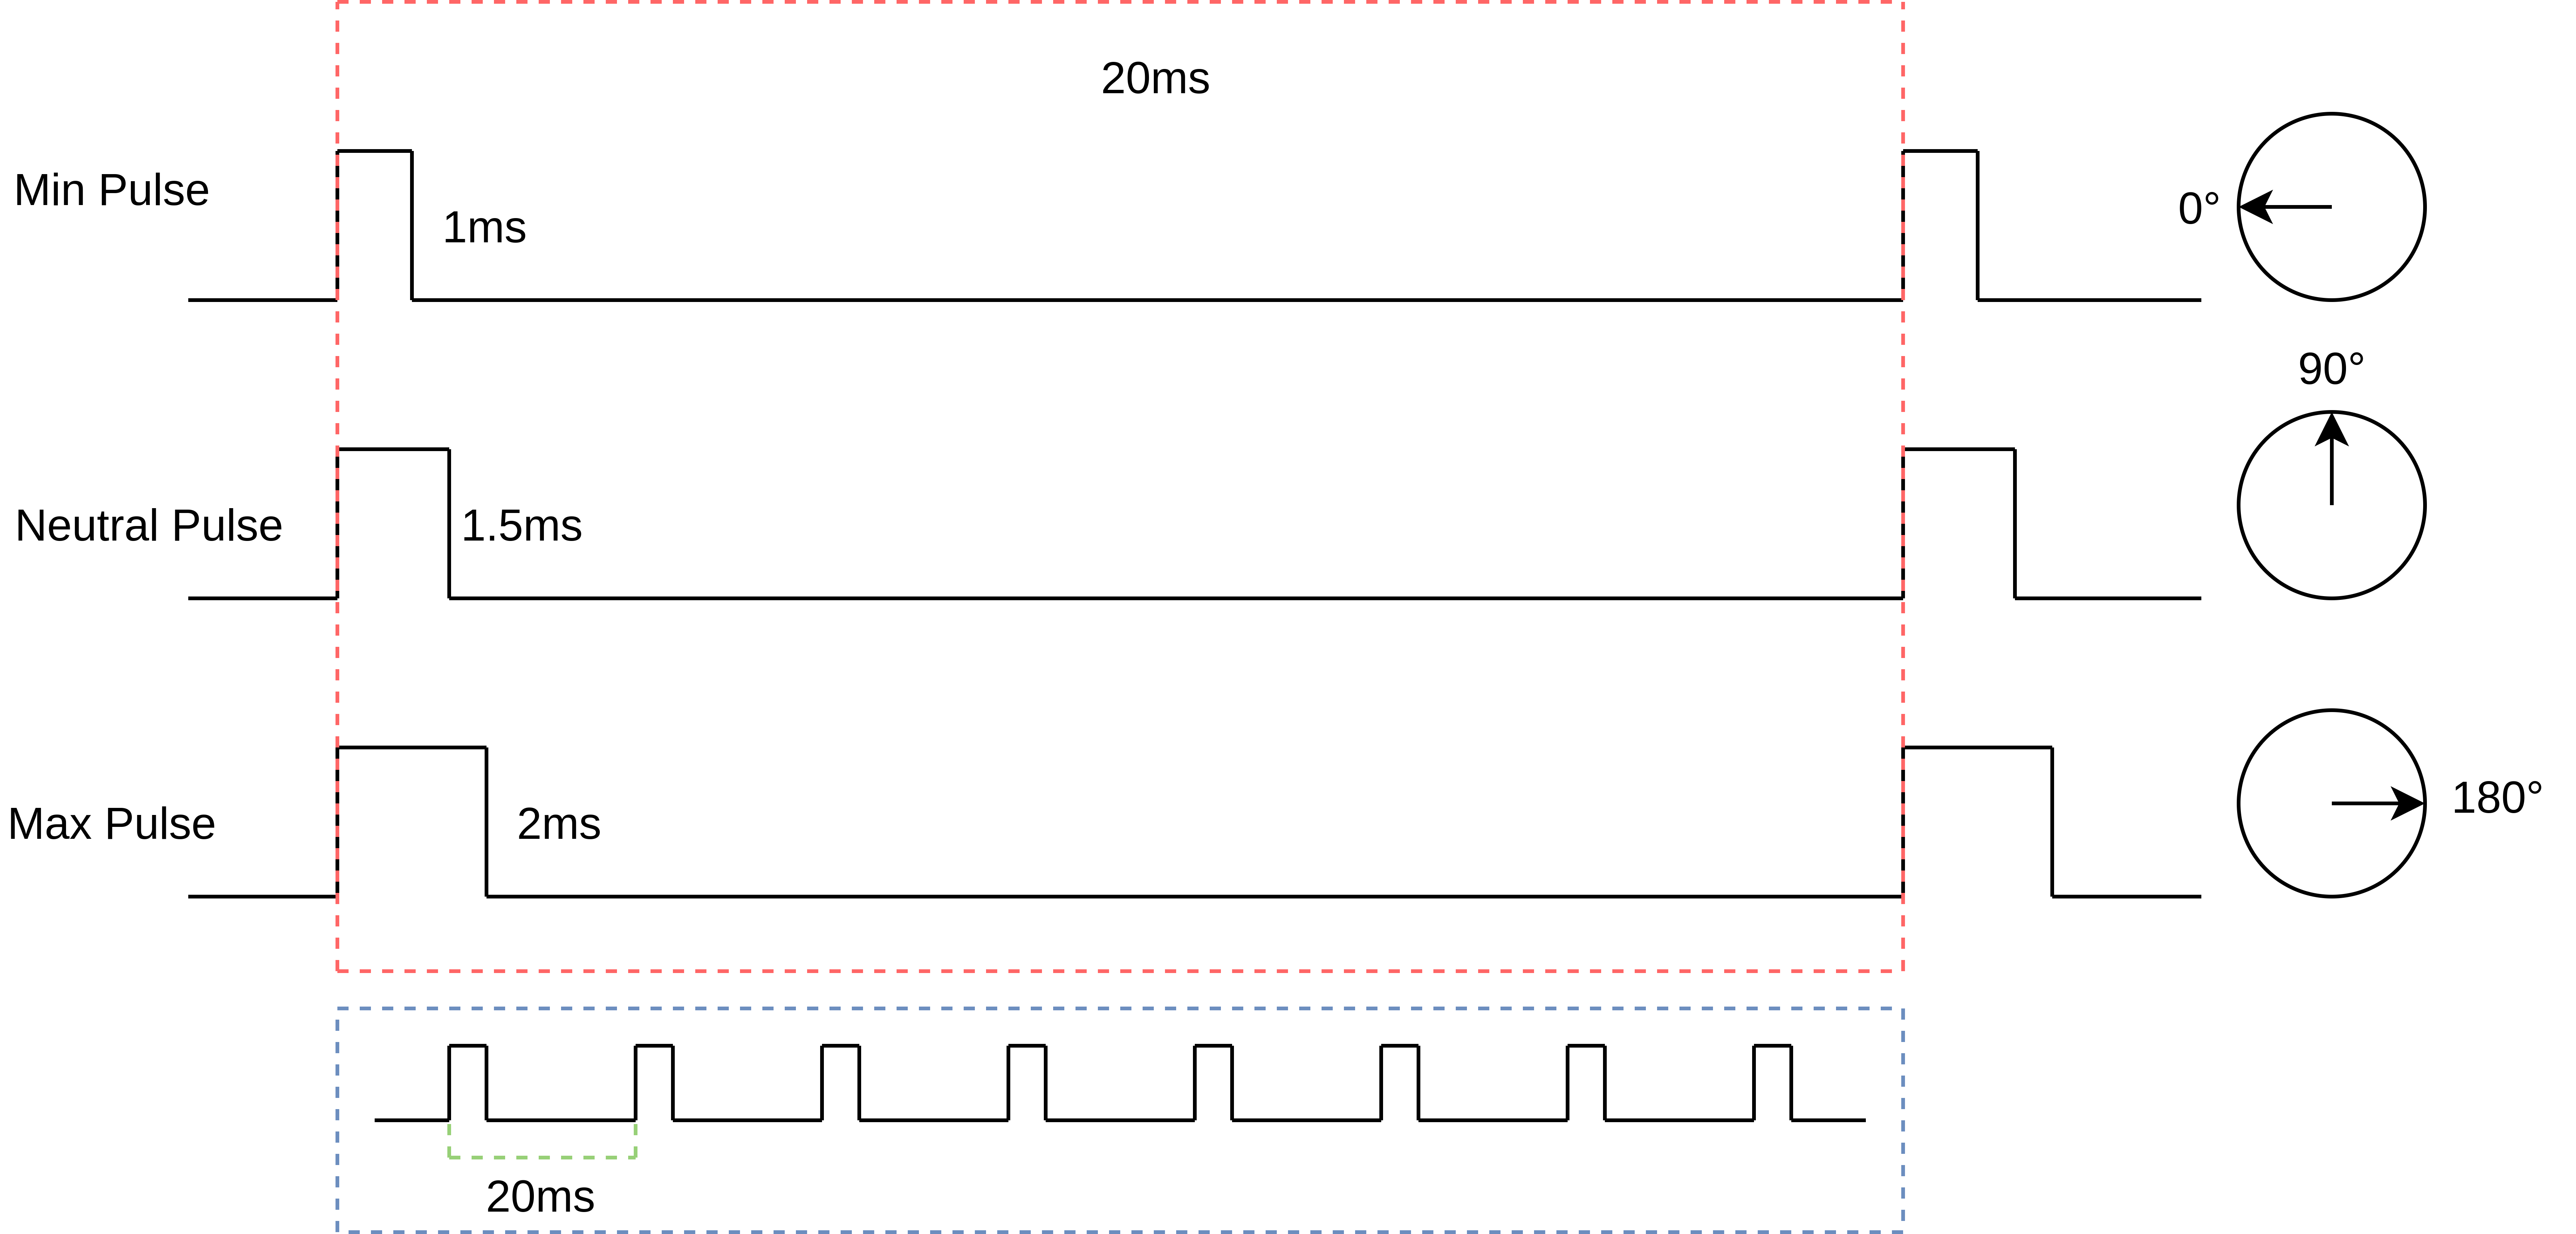
\includegraphics[width=\linewidth]{img/servo.png}
    \end{frame}

    \begin{frame}
        \frametitle{Brushless Motor ESC}
        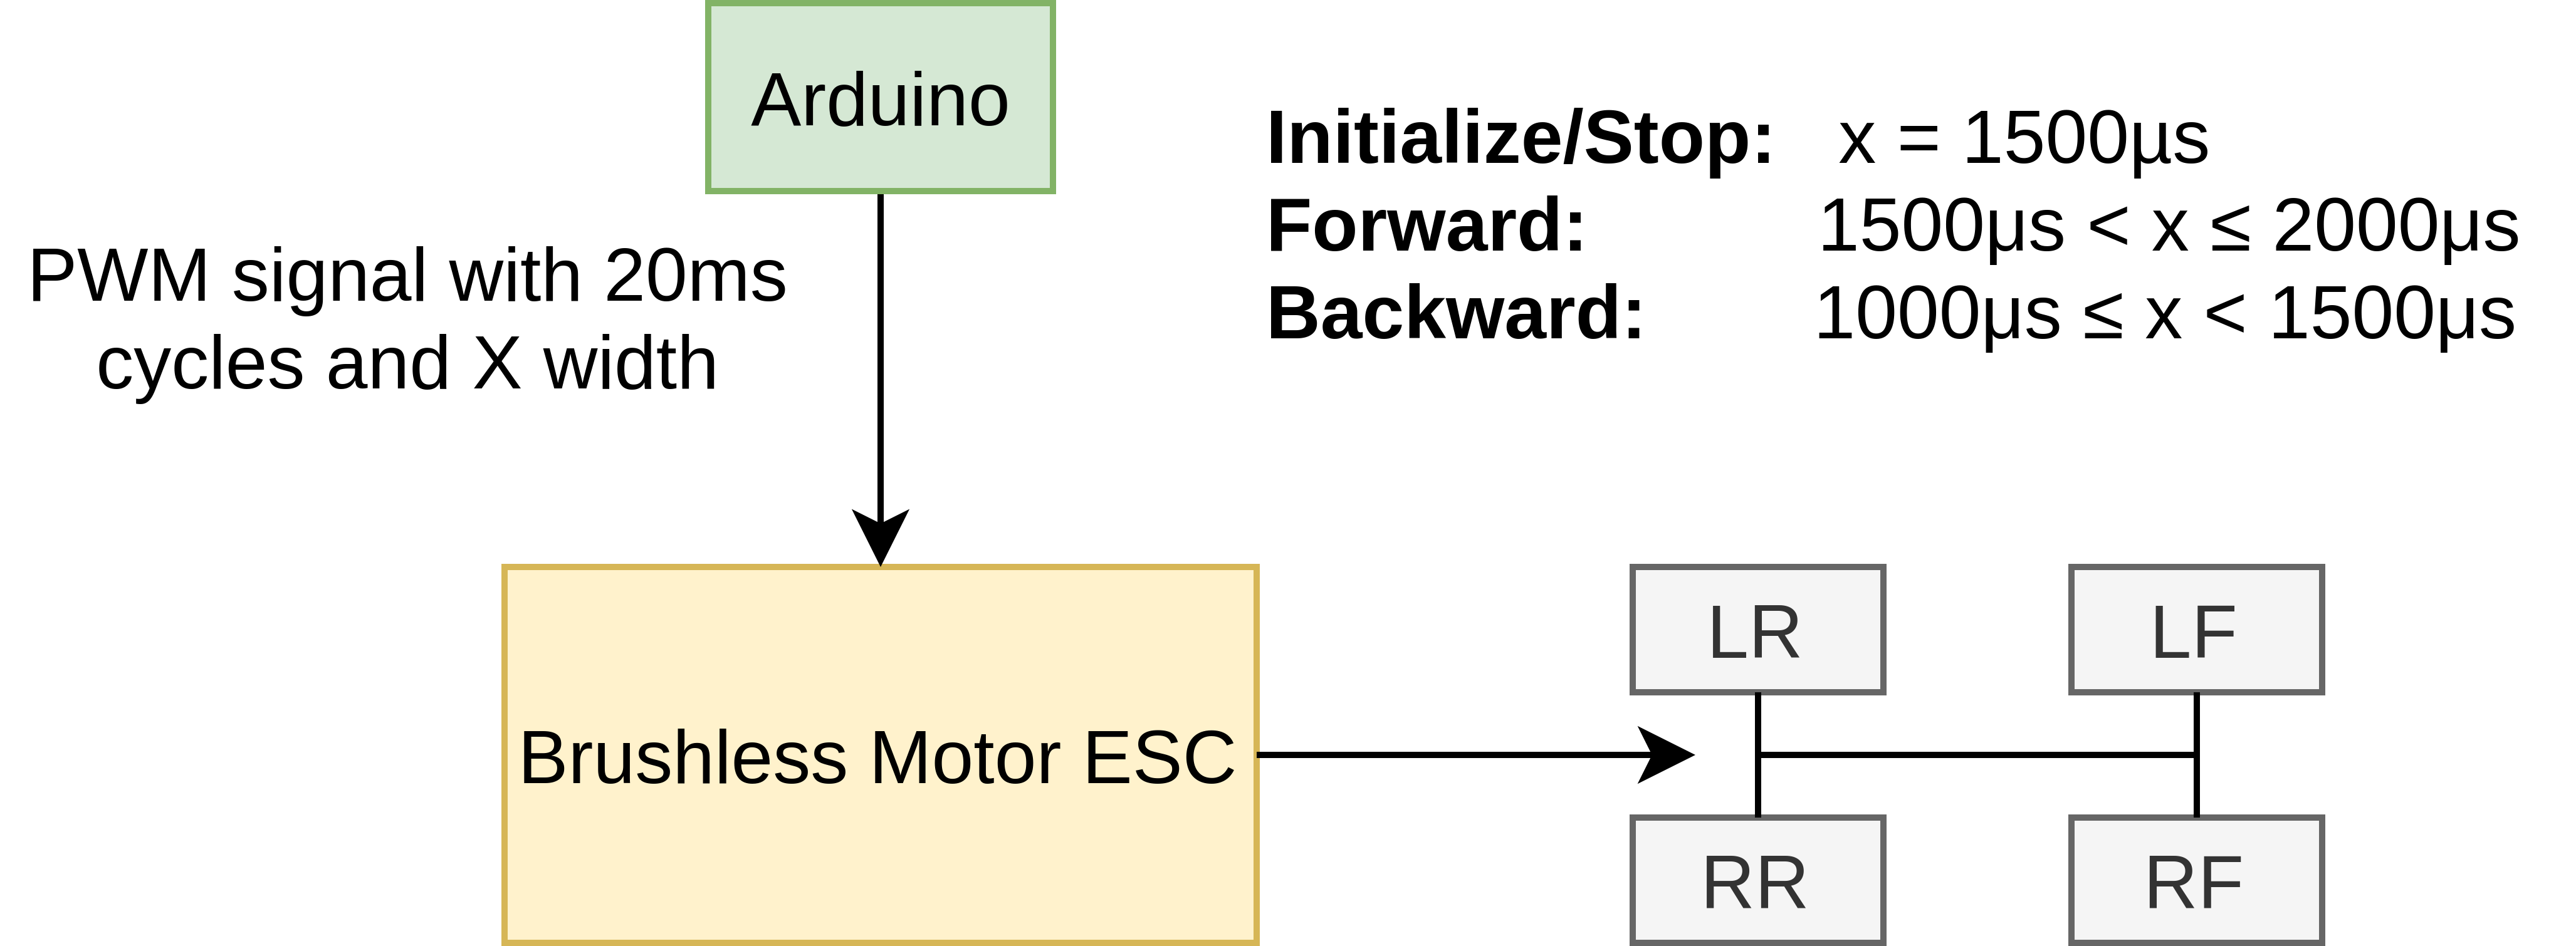
\includegraphics[width=\linewidth]{img/brushless-motor-esc}
    \end{frame}

    \begin{frame}
        \frametitle{Distance Sensor}
        \centering
        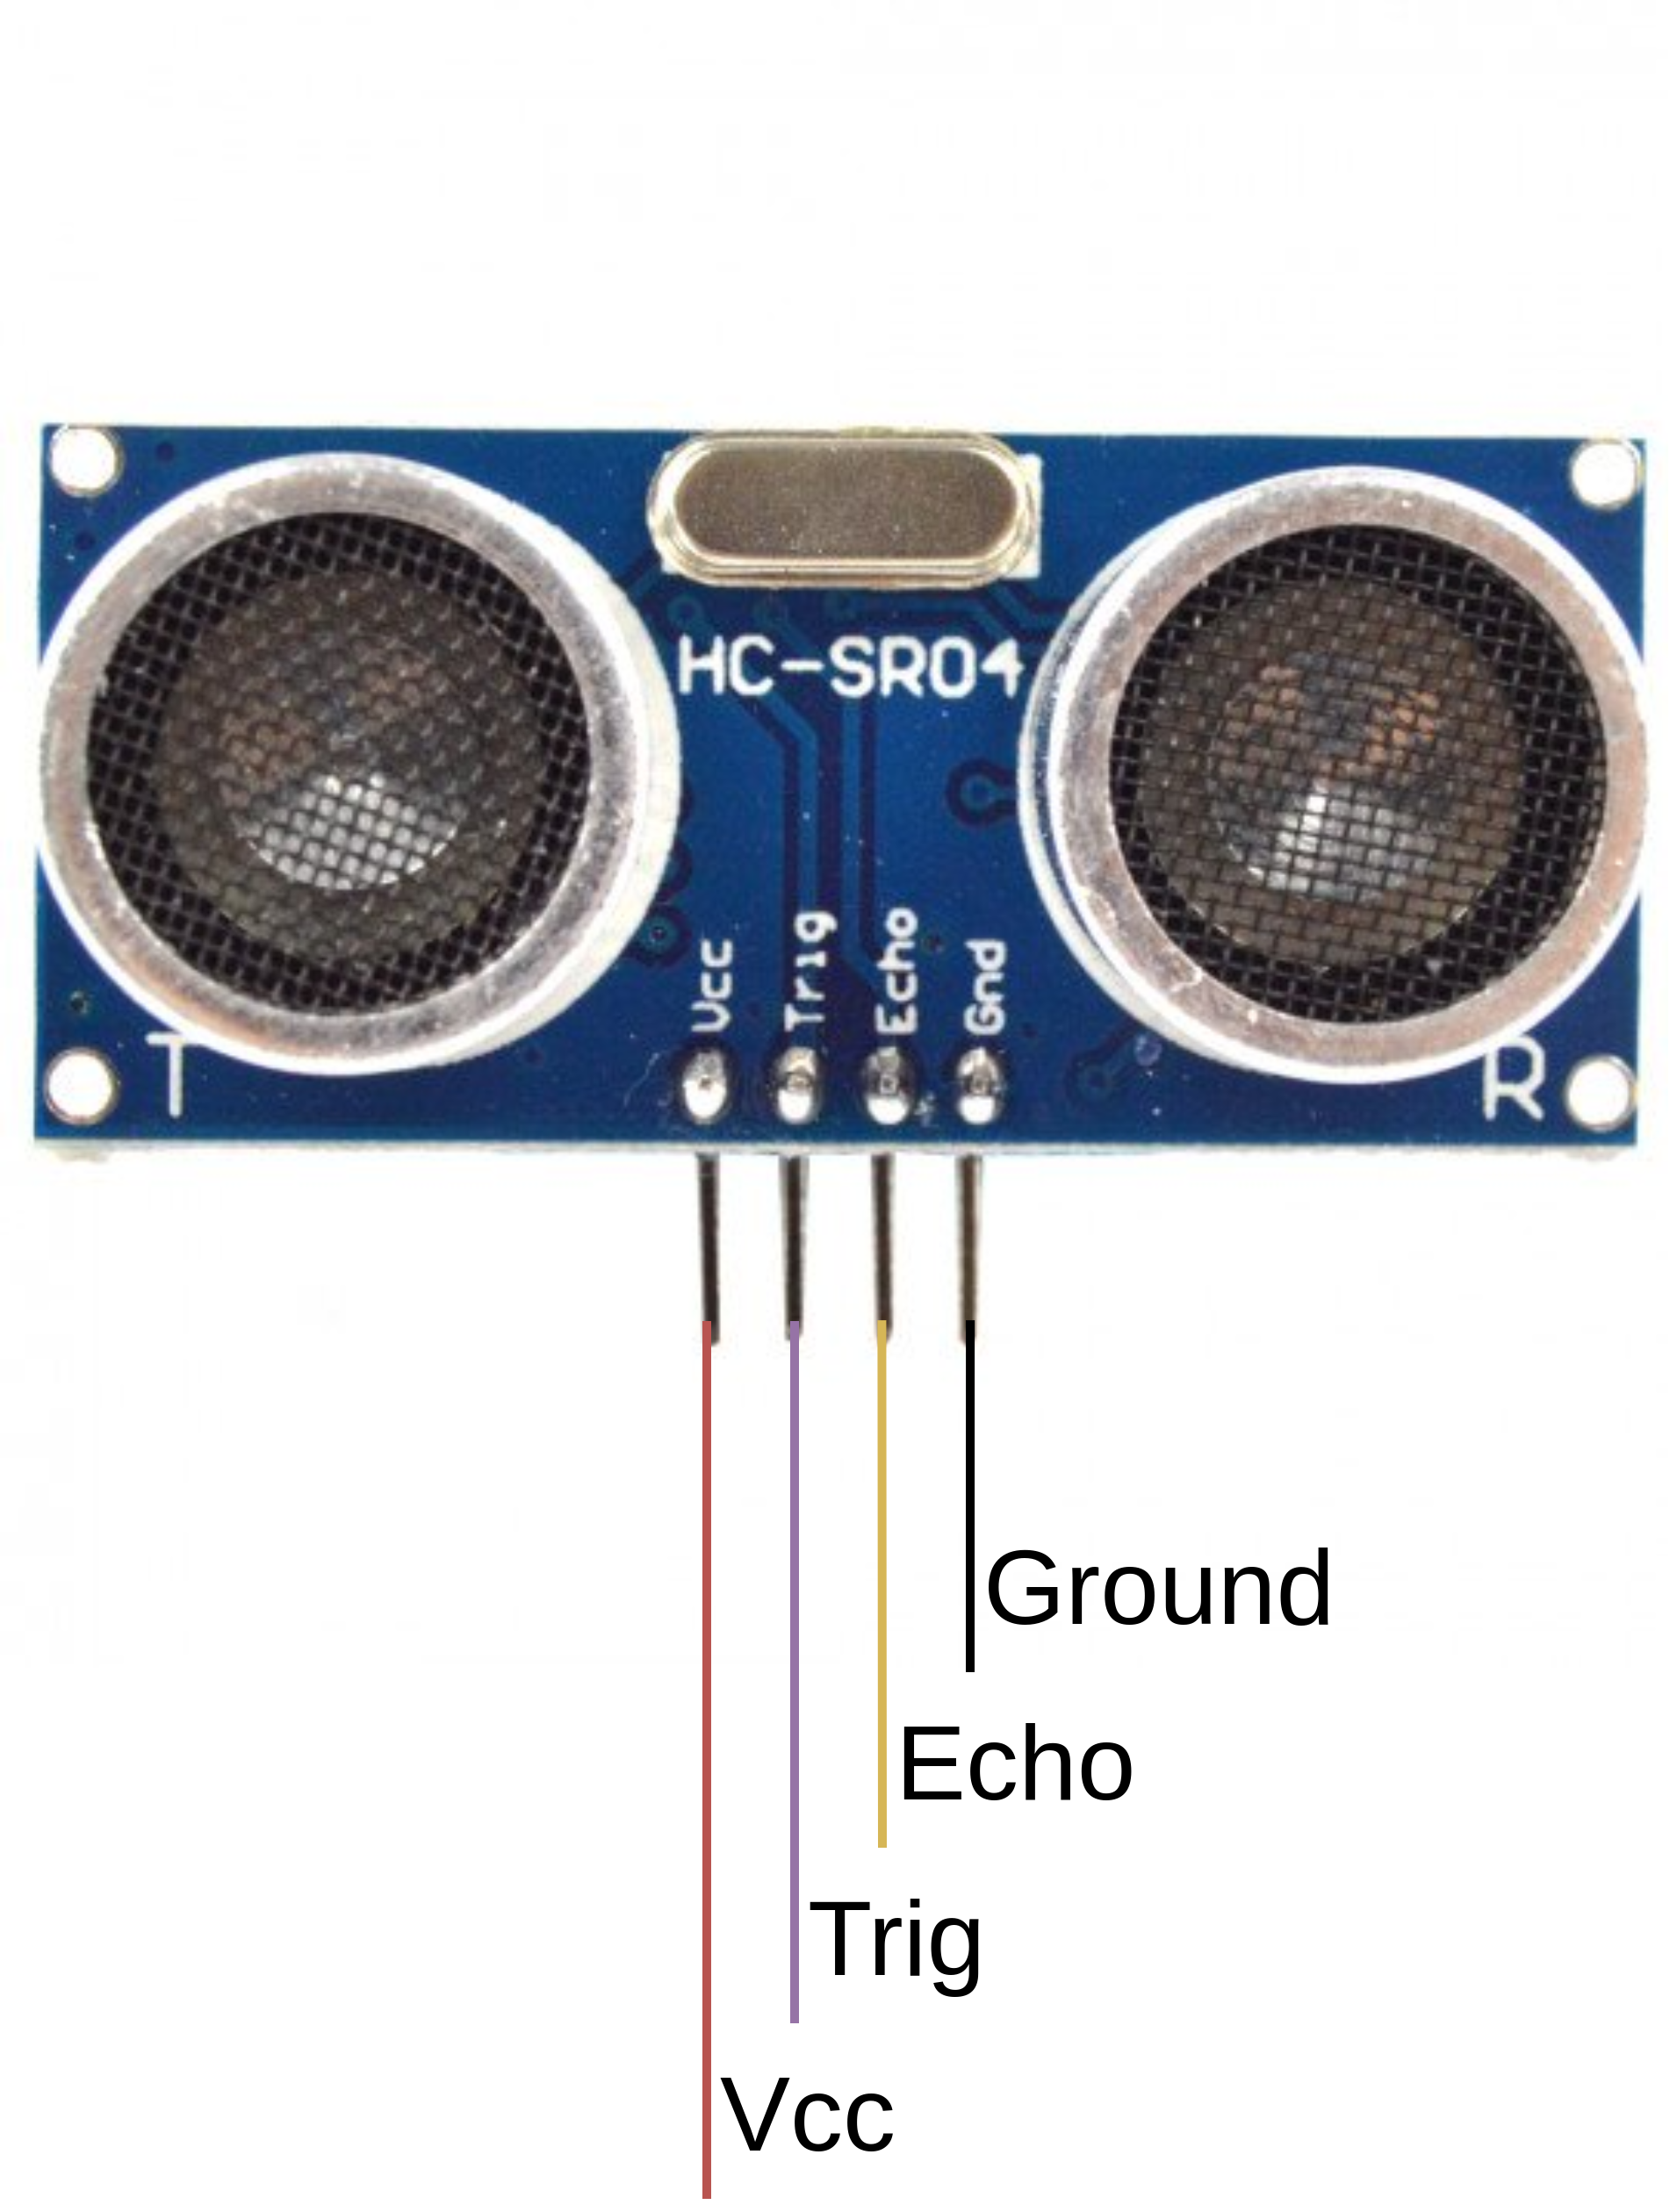
\includegraphics[scale=0.08]{img/hcsr04.png}
    \end{frame}

    \begin{frame}
        \frametitle{Distance Sensor}
        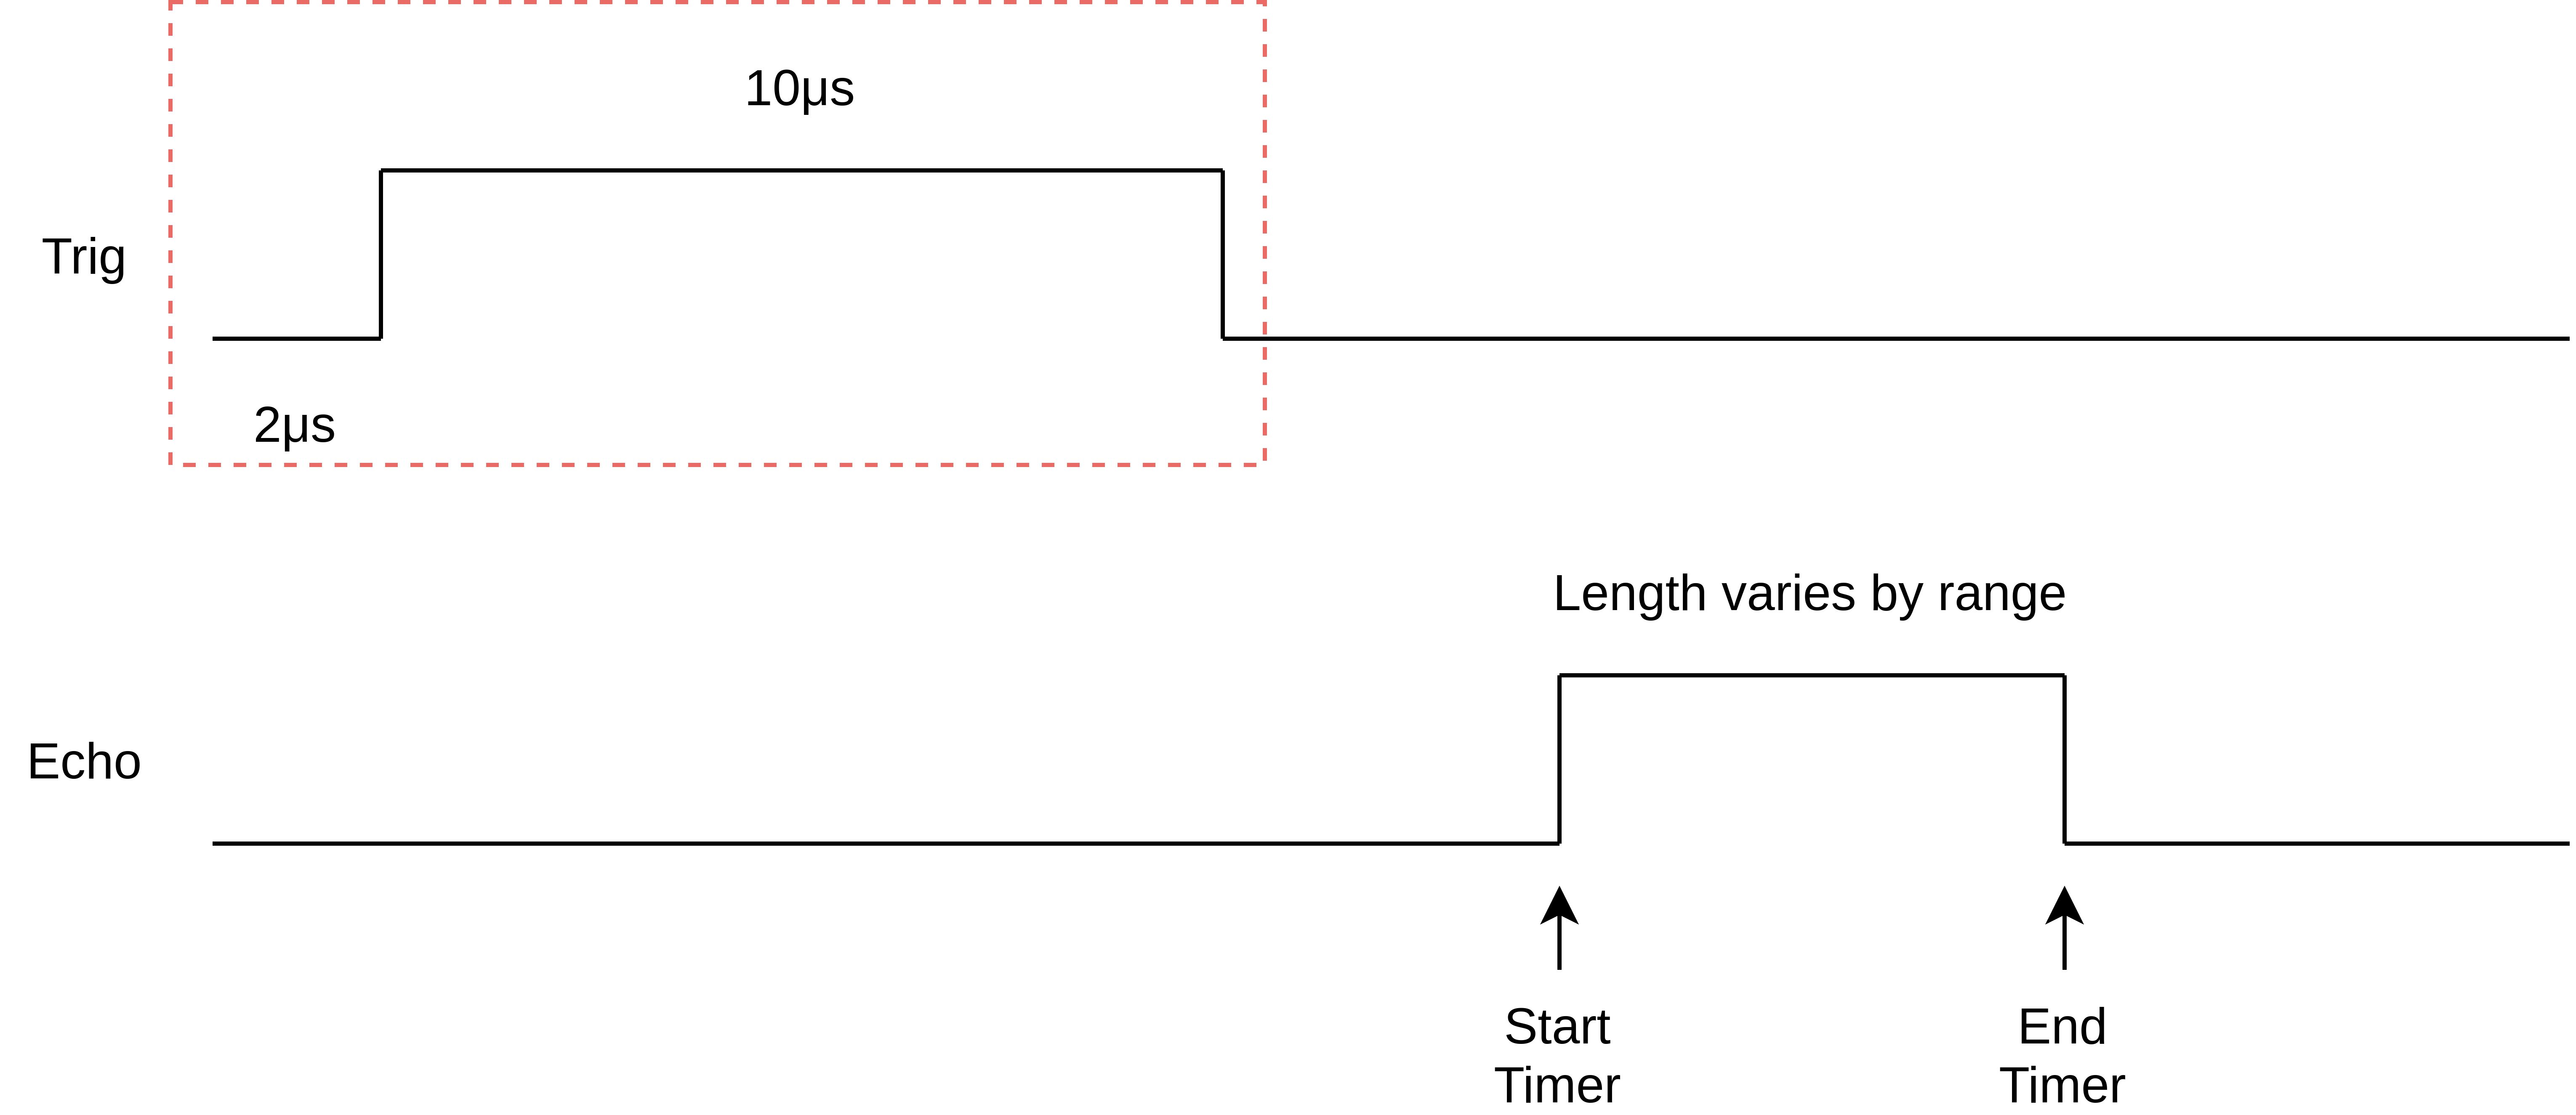
\includegraphics[width=\linewidth]{img/ultrasonic-sensor.png}
    \end{frame}

    \begin{frame}
        \frametitle{System Architecture}
        \centering
        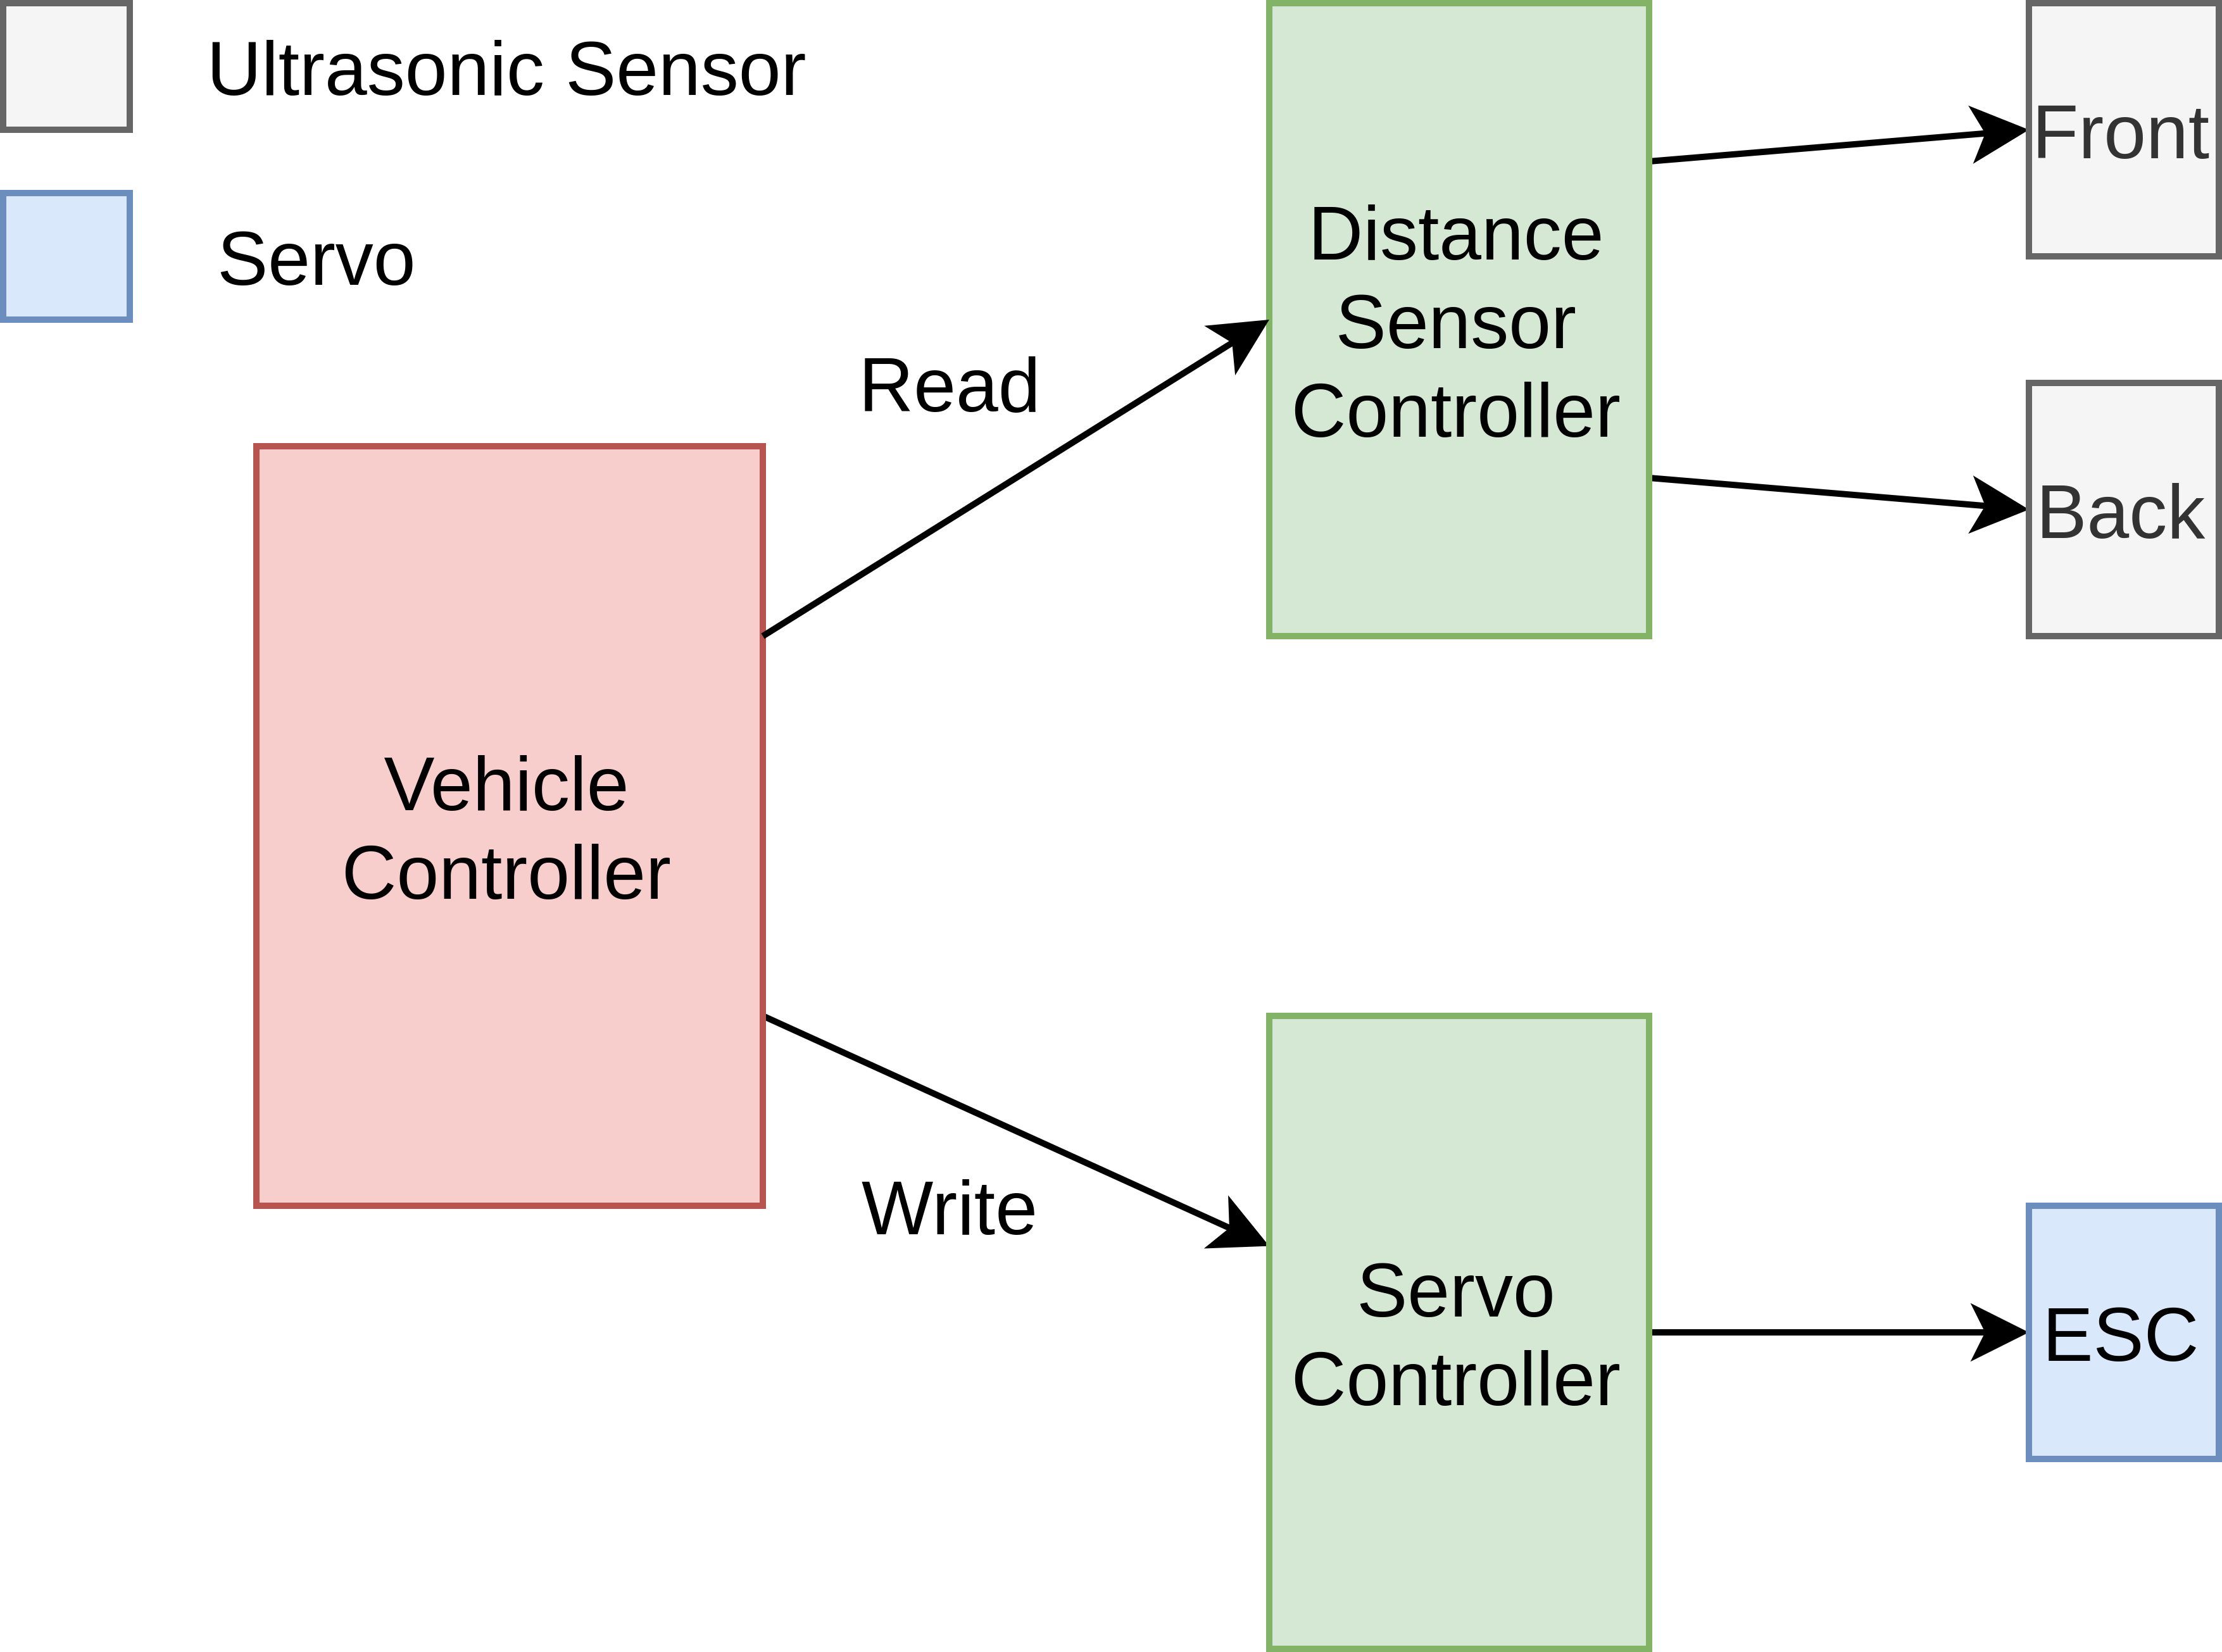
\includegraphics[scale=0.065]{img/system-architecture.png}
    \end{frame}

    \begin{frame}
        \frametitle{Vehicle Controller}
        \centering
        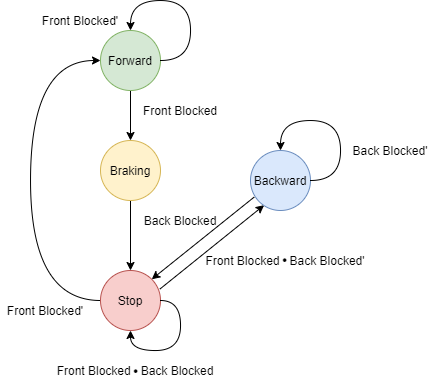
\includegraphics[scale=0.06, keepaspectratio]{img/finite-state-machine.png}
    \end{frame}

    \begin{frame}
        \frametitle{Scheduling with utilization test}
        \begin{center}
            \begin{tabular}{||l l l l|l||}
                \hline
                Task & Period(T) & Comp. time(C) & Priority(P) & Util(U) \\ [0.5ex]
                \hline\hline
                Engine & 20ms & 4094ns & 4 & 0.0002 \\
                \hline
                Compute & 16ms & 844ns & 3 & 0.000052 \\
                \hline
                Sensors & 16ms & 11600190ns & 2 & 0.72 \\
                \hline
                Lights & 200ms & 13438ns & 1 & 0.000067 \\
                \hline
                Main & N/A & 16ns & 0 & 0 \\ [1ex]
                \hline
            \end{tabular}
        \end{center}

        The utilization factor for this system is
        \begin{equation*}
            U_{Sum} = 72.0319\%
        \end{equation*}

        which is lower than the limit of 74.1\% for five tasks.
    \end{frame}

    \begin{frame}
        \centering
        \frametitle{Scheduling with response time analysis}

        \begin{equation*}
            R_{i} = C_{i} + \sum_{j \epsilon hp(i)} \ceil[\Bigg]{\frac{R_{i}}{T_{j}}} C_{j}
        \end{equation*}
        \begin{table}
            \begin{adjustbox}{width=\columnwidth, center}
            \begin{tabular}{||l l l l|l||}
                \hline
                Task & Period(T) & Comp. time(C) & Priority(P) & Response Time(R) \\ 
                \hline\hline
                Engine & 20ms & 4094ns & 4 & 4094ns \\
                \hline
                Compute & 16ms & 844ns & 3 & 4938ns \\
                \hline
                Sensors & 16ms & 11600190ns & 2 & 11605128ns \\
                \hline
                Lights & 200ms & 13438ns & 1 & 11618566ns \\
                \hline
                Main & N/A & 16ns & 0 & N/A \\ 
                \hline
            \end{tabular}
            \end{adjustbox}
        \end{table}
    \end{frame}

    \begin{frame}
        \centering
        \frametitle{Demonstration}
        Live Demo
    \end{frame}

    \begin{frame} 
        \centering
        \frametitle{Questions}
        Any questions?
    \end{frame}

    \begin{frame}
        \centering
        \frametitle{The End}
        Thank you for your attention. :)\\
        You can find our Ada\_Drivers\_Library fork and the source code over at https://github.com/stykk-gruppen
    \end{frame}

\end{document}

